\question{Рентгеновский лазер с ядерной накачкой}

\emph{Лазер с ядерной накачкой} -- это лазерное устройство, возбуждение 
активной среды которого происходит за счет ядерного излучения (гамма-кванты, 
ядерные частицы, продукты ядерных реакций). Длина волны излучения такого 
устройства может быть от дальнего ИК-диапазона до рентгеновского. Одним из 
таких лазеров является рентгеновский лазер с ядерной накачкой, основная 
энергия лазерного излучения которого генерируется в рентгеновском диапазоне 
электромагнитного излучения. Существующие рентгеновские лазеры приводятся в 
действие различными способами, основными из которых являются ядерный либо 
термоядерный взрыв, инверсное излучение возбуждённых плазменных сред, 
излучение возбуждённых твердотельных сред либо синхротронное излучение пучка 
электронов при пролёте через область переменного магнитного поля.

Типы рентгеновских лазеров: \\
1) рентгеновские лазеры с <<накачкой>> от ядерного реактора \\
2) рентгеновский лазер с <<накачкой>> ядерным взрывом

Чтобы осуществлялся эффект усиления электромагнитного излучения при его 
прохождении через активную среду, необходимо, во-первых, большое количество 
возбужденных атомов, готовых испустить кванты вынужденного излучения, а 
во-вторых, большая вероятность взаимодействия между квантами и этими атомами, 
обеспечивающая это вынужденное излучение. Коэффициент усиления излучения 
составляет: \( K = S(N_\text{воз} - N_\text{oсн}) \), где \( S \) -- сечение 
взаимодействия квантов с атомами, \( N_\text{воз} \) и \( N_\text{осн} \) -- 
число атомов в возбужденном и основном состояниях. В условиях 
термодинамического равновесия \( N_\text{воз} < N_\text{oсн} \), поэтому 
поглощение преобладает над вынужденным излучением.

Для получения лазерного эффекта необходимо создать среду с инверсной 
заселенностью атомов по энергетическим состояниям: 
\( N_\text{воз} > N_\text{oсн} \). Из фундаментальных законов квантовой физики 
следует, что чем короче длина волны излучения, тем труднее осуществить его 
квантовое усиление.

Для поддержки инверсной заселенности верхних уровней мощность возбуждения 
должна быть намного больше той, которая рассеивается в виде спонтанного 
излучения в среде (тепловые потери и др). Как известно, энергия кванта 
пропорциональна частоте излучения и к, тому же вероятность спонтанного 
излучения, бесполезно уносящего энергию внешнего источника возбуждения, 
пропорциональна третьей степени от частоты излучения. 

Лазер с накачкой от ядерного взрыва представлен на рис.~\ref{img28.1}. 
Пучок фокусируется в узкую линию (\( d \cong 200 \) мкм, 
\( l = 1.2 \) см) на тонкую (75 нм) полоску селена. Благодаря высокой 
интенсивности пучка накачки (\( \sim 5\cdot10^{13} \text{Вт}/{см}^2 \)) 
фольга взрывается и возникает плазма высокоионизированного селена. Неупругие 
столкновения с электронами горячей плазмы (\( T_E \cong 1 \) кэВ) приводят 
к возбуждению иона \( Se^{24+} \) из основного состояния в возбужденное, и 
между переходами \( 2p^5 3p \) и \( 2p^5 3s \) возникает инверсная 
населенность.

\begin{figure}[h!]
    \center
    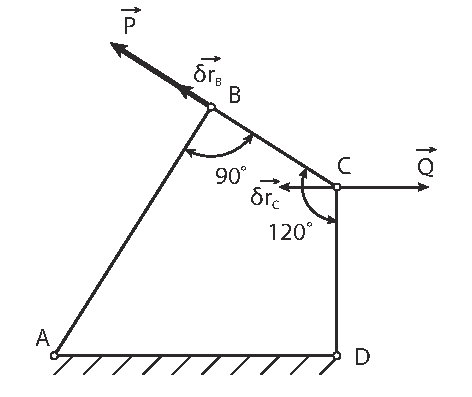
\includegraphics[width=.4\textwidth]{28_01}
    \caption{Геометрия мягкого рентгеновского лазера с поперечным 
    	освещением с использованием метода взрывающейся фольги}
    \label{img28.1}
\end{figure}

Со временем представления первого рентгеновского лазера генерация лазерного 
излучения была получена на многих активных средах, а именно на неоноподобных 
ионах (от \( Ag^{37+} \) до \( Ar^{8+} \)), а также на многих водородоподобных 
(от \( Al^{12+} \) до \( C^{5+} \)), литиеподобных (от 
\( Si^{11+} \) до \( Al^{10+} \)) и на никельподобных ионах 
(от \( Au^{51} \) до \( Eu^{35+} \)). Получена генерация в диапазоне длин волн 
от \( \sim 3.6 \) до \( 47 \) нм, при усилении за проход от \( 10 \) до 
\( 10^3 \).